\usetikzlibrary{positioning}

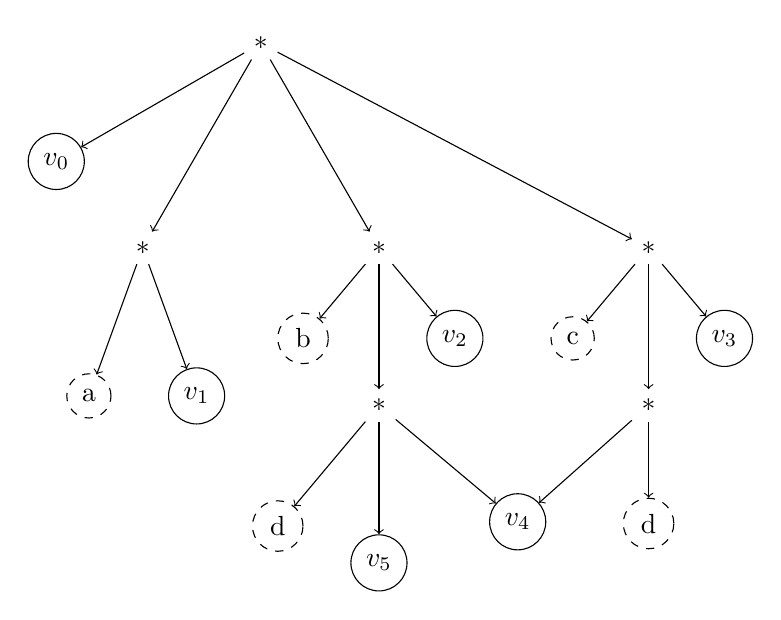
\begin{tikzpicture}[->,circ/.style={draw,circle},node distance=.8cm]

\node (agg0) {$*$};

\path (agg0) ++(-150:3) node[circ] (0) {$v_0$};

\path (agg0) ++(-120:3) node (agg1) {$*$} ++(-110:2) node[dashed,circ] (a) {a};
\path (agg1) ++(-70:2) node[circ] (1) {$v_1$};

\path (agg0) ++(-60:3) node (agg2) {$*$} ++(-130:1.5) node[dashed,circ] (b) {b};
\path (agg2) ++(-50:1.5) node[circ] (2) {$v_2$};
\path (agg2) ++(-90:2) node (agg4) {$*$};

\path (agg4) ++(-130:2) node[dashed,circ] (d2) {d};
\path (agg4) ++(-90:2) node[circ] (5) {$v_5$};
\path (agg4) ++(-40:2.3) node[circ] (4) {$v_4$};

\node[right = 3cm of agg2] (agg3) {$*$};
\path (agg3) ++(-130:1.5) node[dashed,circ] (c) {c};
\path (agg3) ++(-50:1.5) node[circ] (3) {$v_3$};
\path (agg3) ++(-90:2) node (agg5) {$*$} ++(-90:1.5) node[dashed,circ] (d3) {d};

\path[every node/.style={font=\footnotesize,fill=white}]
(agg0) edge (0)
	edge (agg1)
	edge (agg2)
	edge (agg3)
(agg1) edge (a)
	edge (1)
(agg2) edge (b)
	edge (2)
	edge (agg4)
(agg3) edge (c)
	edge (3)
	edge (agg5)
(agg4) edge (d2)
	edge (4)
	edge (5)
(agg5) edge (d3)
	edge (4)
;

\end{tikzpicture}